\documentclass[11pt,a4paper]{report} % Creation d'un rapport avec : 
% taille police : 10 pt
% format : document a4
% optionnel : twocolumn

% Définition des encodages utilisés
\usepackage[T1]{fontenc} % encodage utilisé pour l'impression de caractères (dans le .pdf)
\usepackage[utf8]{inputenc} % encodage utilisé pour la saisie du document (dans le .tex)
\usepackage{lmodern} % utilise la police vectorielle (utile lors d'une impression papier du document) -> c'est plus joli

% Module pour inclure des images 
\usepackage{graphicx} % Pour l'affichage de base

%Gestion des hyperliens
\usepackage{hyperref}

\usepackage{tasks}

%Delete Chapter mention
\usepackage{titlesec}
\titleformat{\chapter}{\normalfont\huge}{\thechapter.}{20pt}{\huge\it}

% Module pour inclure des algorithmes implémentés
\usepackage{listingsutf8} % listings peut faire l'affaire. Celui ci gère mieux les problèmes d'encodage. Doit être chargé après babel
\renewcommand{\lstlistingname}{Code} % Permet de modifier le mot utilisé dans la légende

%Set the language
\lstset{language=sh}

% Module pour inclure des algorithmes en pseudo code
%\usepackage[french,onelanguage]{algorithm2e} % Les options permettent d'avoir les mots clés en français

% Module pour insérer des mathématiques
\usepackage{amsmath}
\newcommand\numberthis{\addtocounter{equation}{1}\tag{\theequation}} % Nouvelle commande pour numéroter une équation particulière avec align* (sinon toutes numérotées avec align, ou aucune numérotée avec align*)

% Configuration de la page de garde
\title{Rapport du projet géomatique \\ Map Matching}
\author{Camille Parisel \\ Romain Mazière \\ Julie Marcuzzi \\ Rudolf Millet \\ Loïc Messal \\ Mamady Samassa \\ Hanane Derbouz}
% Génération d'une image de fond en transparence
\usepackage{eso-pic}
\usepackage{transparent}
\newcommand\BackgroundPic{%
	\put(0,0){%
		\parbox[b][\paperheight]{\paperwidth}{%
			\Logos{../images/logo_ensg_transparent}{../images/qgis-logo}
			\vfill
}}
\put(0,0){%
		\parbox[b][\paperheight]{\paperwidth}{%
			\vfill
			\centering
			{
				\transparent{0.5}
\includegraphics[width=0.9\paperwidth,keepaspectratio]{../images/logo_grand.png}}%
			\vfill
}}
}


% Pour les logos
\newcommand{\Logos}[2]{%
\vspace{1cm}
\begin{center}
\hfill
	\begin{minipage}[c]{0.40\paperwidth}
		\begin{center}
			\includegraphics[width=3.5cm, keepaspectratio]{#1}
		\end{center}
	\end{minipage}
	\hfill
	\hspace*{0.19\paperwidth}
	\begin{minipage}[c]{0.40\paperwidth}
		\begin{center}
			\includegraphics[width=2.5cm, keepaspectratio]{#2}
		\end{center}
	\end{minipage}
	\hfill
\end{center}
}


% Configuration de la langue utilisée (pour les mots clés comme "chapitre", pour le découpage des mots à la fin des lignes...)
%\usepackage[french]{babel}

% Module pour inclure des algorithmes implémentés
%\usepackage{listingsutf8} % listings peut faire l'affaire. Celui ci gère mieux les problèmes d'encodage. Doit être chargé après babel
%\renewcommand{\lstlistingname}{Code} % Permet de modifier le mot utilisé dans la légende

% Module pour régler les marges du document
\usepackage[left=2cm,right=2cm,top=2cm,bottom=2cm]{geometry}


\begin{document}

\begin{titlepage}
		
	\~ 
	\newline
	\\[2cm]
	\newcommand{\HRule}{\rule{\linewidth}{0.5mm}} % Defines a new command for the horizontal lines, change thickness here
		
	\center % Center everything on the page
		
	%----------------------------------------------------------------------------------------
	%	HEADING SECTIONS
	%----------------------------------------------------------------------------------------
		
	\textsc{\LARGE \'Ecole Nationale des Sciences Géographiques}\\[0.5cm] % Name of your university/college
	\textsc{\Large Master Technologies des Systèmes d'Informations}\\[0.5cm] % Major heading such as course name
	%----------------------------------------------------------------------------------------
	%	TITLE SECTION
	%----------------------------------------------------------------------------------------
		
	\HRule \\[0.4cm]
	{ \huge \bfseries Geomatic project report}\\[0.4cm] % Title of your document
	\HRule \\[1.5cm]
	\vfill
	%----------------------------------------------------------------------------------------
	%	AUTHOR SECTION
	%----------------------------------------------------------------------------------------
		
	\begin{minipage}[t]{0.4\textwidth}
		\begin{flushleft} \large
			\emph{Authors : } \newline \\
			Camille \textsc{Parisel} \\ 
			Romain \textsc{Mazière} \\ 
			Julie \textsc{Marcuzzi} \\ 
			Rudolf \textsc{Millet} \\ 
			Loïc \textsc{Messal} \\ 
			Mamady \textsc{Samassa} \\ 
			Hanane \textsc{Derbouz}
						
		\end{flushleft}
	\end{minipage}
	~
	\begin{minipage}[t]{0.4\textwidth}
		\begin{flushright} \large
			\emph{Supervisors : \\ \ \\ } 
			Didier \textsc{Richard} \\
			Benoît \textsc{Costes} \\
		\end{flushright}
	\end{minipage}\\[1cm]
		
	%----------------------------------------------------------------------------------------
	%	DATE SECTION
	%----------------------------------------------------------------------------------------
		
	{\large \today}\\[2cm] % Date, change the \today to a set date if you want to be precise
		
	%----------------------------------------------------------------------------------------
	%	LOGO SECTION
	%----------------------------------------------------------------------------------------
		
	%\includegraphics{Logo}\\[1cm] % Include a department/university logo - this will require the graphicx package
		 
	%----------------------------------------------------------------------------------------
		
		
	\AddToShipoutPicture*{\BackgroundPic} % Genere une image de fond
	%\AddToShipoutPicture*{\Logos{images/logo_crg}{images/logo_ensg_transparent}}
\end{titlepage}




\ClearShipoutPictureBG % Supprime l'image en fond
%\tableofcontents
%\listoffigures
%\listoftables
%\listofalgorithms

%\part{Contexte}
C'est quand même important de commencer par présenter le contexte du travail.
\chapter{Introduction}
Ici nous venons de créer un nouveau chapitre.
\section{Pourquoi cette formation}
Parce que Latex va vous permettre de rédiger un document en équipe, sans se soucier des préférences d'affichage. Latex sera respectueux de l'utilisation de votre système d'exploitation. Il est utilisable que vous soyez sous windows, sous mac ou sous linux.
\subsection{Le lieu}
Durant votre scolarité à l'ENSG, vous allez rédiger bon nombre de rapports. 
\subsubsection{Vertigeo dans tout ça}
Parce que faire de la pub pour la Junior Entreprise, c'est cool.
\paragraph{Rédigé, c'est structuré}
La mise en forme est gérée par Latex, on peut donc en théorie se concentrer sur le contenu du rapport.
\subparagraph{Toujours plus}
Un niveau en dessous du paragraphe. Cela peut être utile dans certaines situations

L'intérêt de cette formation est de vous initier à Latex. Car bien qu'il permet de se concentrer sur le contenu, si son fonctionnement n'est pas compris, ou si personne ne vous a montré un exemple, vous allez passer plus de temps à gérer un problème de mise en forme plutôt qu'écrire du contenu. (Exemple d'une image)

\subsection{Une autre subsection}
Celle ci est vide. Remarquez que le numéro s'est mis à jour.
\section{Quelques conseils}
La table des matières est mise à jour après deux compilations sans modification de la structure entre temps. La première compilation permet à Latex de savoir quelles vont être les entrées. Le deuxième passage va l'afficher.
\subsection*{Structure non numérotée}
Pour ajouter une structure qui n'apparaît pas dans la légende, il suffit de rajouter * après la commande. En faisant ceci, Latex ignorera cette entrée, ce qui signifie pas de numéro, ni de place dans la table des matières. Peut être pratique pour une section Introduction ou Conclusion par exemple.

\subsection{Mettre en valeur des éléments}
Le texte peut être mis en valeur par quelques commandes. Il est possible de \textbf{mettre en gras}, \emph{mettre en italique}.

\section*{Conclusion}
\addcontentsline{toc}{section}{Conclusion}
(Cette entrée apparaît dans la table des matières.)
Au final, nous avons appris quelque chose. Je connais maintenant la base de Latex. Il m'a fallu quelques heures de formation. Je peux désormais rédiger des rapports qui font pro. Je suis content.

\part{Quelques éléments utiles}
\section{Les listes}
Les listes non numérotées : 
\begin{itemize}
	\item Exemple de liste non numérotée
\end{itemize}

Et les listes numérotées : 
\begin{enumerate}
	\item Exemple de liste numérotée
	\item Celle-ci a deux éléments
\end{enumerate}
Notez que le début des paragraphes sont indentés. Ils se retrouvent donc au même \og{}niveau\fg{} que la puce des listes. Ah la langue française\dots
\section{Insérer une image}
Il est possible d'ajouter des images et de les redimensionner par rapport à la dimension du papier, comme la figure \ref{format}.
La référence est mise à jour automatiquement et est associée au label de même nom (se trouvant dans la légende de l'image. Comme pour la table des matières, cela nécessite plusieurs compilations.
\begin{figure}[!ht]
	\begin{center}
		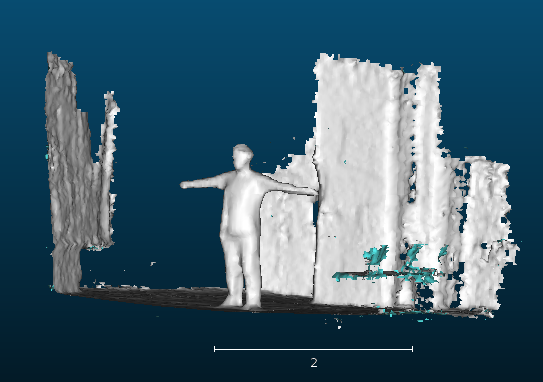
\includegraphics[width=0.50\linewidth, keepaspectratio]{../images/format.png}
		\caption{Format obj sans texture \label{format}}
	\end{center}
\end{figure}
  
\section{Insérer un tableau}
\begin{table}[!ht]
	\begin{center}
		\begin{tabular}{rl|c}
			Prenom & Nom      & Promotion \\
			Jean   & Aymare   & 2014      \\
			Jean   & Peuplus  & 2015      \\
			José  & Paledire & 2016      \\
		\end{tabular}
		\caption{Un joli tableau \label{tableau}}
	\end{center}
\end{table}
\section{Insérer des algorithmes}
Voici un exemple d'algorithme en pseudo code : 

\begin{algorithm}[H]
	\SetAlgoLined
	\KwData{Ce document}
	\KwResult{Être capable de rédiger un rapport en Latex }
	initialisation\;
	\While{non à la fin de la formation}{
		Continuer d'écouter\;
		\eIf{compris}{
			Essayer par soit même\;
			Aider ceux qui en ont besoin\;
			}{
			Poser des questions\;
		}
	}
	\caption{Bien suivre la formation}
\end{algorithm}
\section{Insérer du code}
L'option \emph{frame} permet de jouer sur la bordure.
\begin{lstlisting}[language=Python, frame=L, caption={Une imprimante des premiers nombres},label=monImprimante]  % Start your code-block

def printer():
	for i in range(10):
		print(i)
	return true
\end{lstlisting}

\begin{lstlisting}[language=Python, frame=single, caption={Une seconde imprimante des premiers nombres},label=monImprimante2]  % Start your code-block

def printer():
	for i in range(10):
		print(i)
	return true
\end{lstlisting}

\begin{lstlisting}[language=Python, frame=shadowbox, caption={Une troisième imprimante des premiers nombres},label=monImprimante3]  % Start your code-block

def printer():
	for i in range(10):
		print(i)
	return true
\end{lstlisting}


\section{Insérer des formules mathematiques}
Il est possible d'écrire des formules mathématiques intégrées dans le texte, comme \begin{math}(a-b)^2=a^2-2ab+b^2\end{math} ou en utilisant la notation condensée $(a+b)^2=a^2+2ab+b^2$.

De la même façon, il est possible de séparer les formules mathématiques pour les rendre plus visibles :
\begin{displaymath}
	det \begin{pmatrix}
	\alpha & \beta \\
	\gamma & \delta
	\end{pmatrix} = \alpha\delta - \gamma\beta 
\end{displaymath} ou dans sa notation abrégée : 
$$
\begin{vmatrix} 
	a & b \\
	c & d 
\end{vmatrix} = ad - cb
$$

On peut même utiliser une structure similaire à la précédente et qui permet de numéroter les équations : \begin{equation}
\sin x=\sum_{k=0}^{\infty}\frac{(-1)^k}{(2k+1)!}x^{2k+1}
\end{equation}
\begin{align*}
	\int_a^b x^2 \, \mathrm dx & = {\lbrack \frac{x^3}{3} \rbrack}_a^b                     \\
	                           & = \frac{b^3}{3} - \frac{a^3}{3}                           \\
	                           & = \frac{b^3-a^3}{3} \numberthis \label{resultatIntegrale} 
\end{align*}
L'équation \eqref{resultatIntegrale} montre que le résultat de l'intégrale est calculable.
\medbreak
Latex génère aussi les flèches pour les vecteurs. Avec ça, on a quasiment tout ce qu'il nous faut pour faire des maths.
$$
\overrightarrow{\nabla }=\frac{\partial }{\partial x}\overrightarrow{i}+\frac{\partial }{\partial y}\overrightarrow{j}+\frac{\partial }{\partial z}
\overrightarrow{k}
$$
\chapter{Introduction}
La localisation exacte des biens et des personnes est un enjeu fondamental du XXI\ieme siècle. L'aide à la navigation est l'une des applications de la localisation. Elle a permis d'optimiser des trajets aussi bien commerciaux que personnels.
\section{Présentation du projet}
\subsection{Contexte}

\subsection{Objectif}
L'objectif de ce projet est de développer un outil de recalage de traces GPS. Cela inclut :
\begin{itemize}
\item{} un processus de map matching pour un lot de traces GPS
\item{} un processus de map matching pour une acquisition en temps réel
\item{} une interface graphique pour visualiser les données 3D (traces, réseau routier, fond de carte, \dots)
\end{itemize}
\subsection{Ressources}

\subsection{\'Equipe}
\subsection{Outils utilisés}
\chapter{Gestion du projet}
\section{Méthodologie agile}
\section{Outils utilisés}
%\chapter{Algorithme}
Ceci est l'explication de notre algorithme.
%\chapter{Conclusion}
Ceci est notre conclusion.
\chapter{Project implementation}

\section{Presentation of the Map-Matching method}

The objective is to match GPS points to roads by constructing a Hidden Markov Model with roads as states and GPS points as observations. Once the Hidden Markov Model is built, a dynamic programming technique, called Viterbi algorithm, is applied to find the most probable sequence of roads.

The paper (ref) presents how the matrices of the HMM are built and the robustness of the algorithm with different time steps for the GPS track.

The emission matrix $E$ reports the probabilistic relation between a point and the surrounding roads (up to 200m). 
The closer the point $p$ is to a road $r$ the higher the probability $E(p,r)$ is.
	
The transition matrix $M$ reports the probability of going to road $r_j$ from a road $r_i$. In the HMM theory, the probability of transitioning is independent of the observations.

In the paper, this probability depends on the distance between two consecutive points (straight distance) and the distance between the projection of those points on the roads.

A few constants are introduced (but their real value not given in the paper) for the probability computations. For instance, $\sigma_z$ represents the standard deviation of GPS measurements and is part of the computation of the emission matrix.  

\section{Input data}

The map matching algorithms works with GPS points and roads expressed as coordinates (x,y) in the metric system. 
The data presented on the paper is freely available in the latitude and longitude system including other informations such as one-ways and average speed (for roads).

This input data, as well as data from Paris, has been processed through \textbf{QGIS} to produce ready to use datasets :
\begin{itemize}
	\item a full dataset (road network and GPS track) from the paper representing a trip of more than 7500 points in Seattle (2500+ roads);
	\item a small dataset from the same inputs (231 GPS points);
	\item datasets of trips in Paris.
\end{itemize}

For each of these datasets, we have, at least :
\begin{description}
	\item[Tracks] x,y in meters and a timestamp;
	\item[Network] a set of coordinates describing the extremities of each segment of a road.
\end{description}

\section{Implementation hazards}

Once the input data where available in the adequate form (sufficient information expressed in meters), we could focus on the difficulties of the algorithms and the implementations options. 

A basic UML class diagram was produced in order to initiate the agile process. The principle being that each sprint would lead to a prototype expanding the previous sprint's prototype, hence adding more classes and functionalities to the software.

During the development phase, Doxygen was used to generate updated UML class diagrams.

<uml pic>

We have simplified the computation of both the emission matrix and the transition matrix. This was a side effect of our choice to not use a spatial library.

In the end, we were able to get a similar results as the one shown on the paper. Our probabilities don't follow the same distribution and its shows after a long strand of GPS point corrections : as each probability depends on all the previous steps, its value can only go down. Using \textit{double} instead of \textit{float} only delay the moments where the values of all the probabilities for one timestep are almost null.  


\section{Implementation details}

From the project description, we were advised to use C++, OpenGL through a library, QGIS, Globe, and Unit Tests.

A previously mentioned, QGIS has been used to transform input data, and more generally, to visualize tracks and road networks. 

During the first sprint, we focused on getting a grip on C++ QGIS plugins and Globe. Our conclusion was that not only it is very unlikely that we would succeed in compiling the whole QGIS project on Debian\footnote{QGIS includes Globe, so by setting all the required libraries with their correct versions for QGIS, we should have been able to compile Globe.}, but the development of a code as a plug in would drastically slow down our progress. As a stand alone application, it was way easier to detect any bugs and focus on our own code. The drawback is that none of the functionalities of QGIS (like computing distance, selecting roads in an area) where available to us. 

\subsection{Unit tests}

Our development has been done with Qt Creator and a limited use of Qt libraries. Qt offers a Unit Test library (Qt Test). A quick research showed that a large amount of C++ projects uses GoogleTest. We think that it is a better investment to use a well established standard. 
Google Test is relatively easy to setup and use (a short documentation was written to get everyone up to speed). We only tackled a tiny part of the possibilities of GTest as we focused on checking basic functionalities of our code (related to GSP tracks and road segments), but we are confident that we can go deeper on a future project. 

\subsection{Visualization and spatialization}

A big side effect of our decision to not use QGIS was the problem of visualization and more specifically of spatialization.

Qt is a very rich development framework. Among all the libraries, is \textit{GraphicsScene} and \textit{GraphicsView}. Whith those two classes, we could easily display, zoom and navigate on a road network, and, more importantly, take opportunity of its embedded partitioning to quickly select a set of neighboring roads.

\subsection{Other concepts}

In order to have a responsive UI (when loading files and during the visualization of the track correction), we have separated all the GUI classes and the "logic" classes in two threads, a feat easily done in Qt thanks to its Qt thread library.

Communication between threads is performed with the slot/event system provided by Qt.

GUI classes helped to create a user friendly interface. 




\end{document}


